\documentclass[a4paper,12pt]{article}
\usepackage[utf8x]{inputenc}
\usepackage{ucs}
\usepackage[english]{babel}
\usepackage{amsfonts}
\usepackage{amssymb}
\usepackage{amsmath}
\usepackage{hyperref}
\usepackage{graphicx}

\title{Solving CAPTCHAs}
\author{Mihai Maruseac, Lucian Mogoșanu, Sofia Neață, Adrian Șendroiu}
\date{March 2012}

% TODO: use a different template/layout for paper/journal
% TODO: restructure tex if document has the change of getting big
\begin{document}

\maketitle

The repository for this project can be found on GitHub
\footnote{\url{https://github.com/mihaimaruseac/ssl}}.

\section*{Project motivation}

The CAPTCHA (Completely Automated Public Turing test to tell
Computers and Humans Apart) mechanism is a measure widely used on
the World Wide Web to provide tests solvable only by human users.
It is commonly used as a means to prevent problems such as automated
spam, website registration, collection of e-mail addresses or abuse
of services such as online voting.

Usually CAPTCHAs consist of a challenge-response test in which the
user is provided with an image containing a small number of words
and is asked to type them back. This kind of test is in theory
easily solvable by a human agent, while the problem of recognizing the
text in an image is not trivial from the point of view of algorithms.
Moreover, the CAPTCHA usually contains noise and/or distorted text,
making the use techniques such as Optical Character Recognition
difficult. This is similar to the manner in which one-way functions
are used in cryptographic algorithms.

Our project aims to use Machine Learning for the purpose of solving
CAPTCHAs. There are several approaches to this. One approach would
involve using a free/open source CAPTCHA generator to generate
a set of training and/or test examples and try to improve on
various algorithms known to work well on this problem. Testing
against well-known CAPTCHA systems such as Google's reCAPTCHA
\footnote{\url{http://www.google.com/recaptcha}} could also give
us a good idea about the performance of our algorithm(s), as
well as the effectiveness of CAPTCHA as a security mechanism.

\section*{State of The Art}

CAPTCHA tests can be found in various forms on the Internet, ranging
from short audio streams to images. Thus previous research on the
matter has been focused more or less on all these aspects. For
example Tam et al. \cite{VonAhn_Tam_Hyde_Simsa_2009} use a technique
similar to a Fast Fourier Transform (FFT), along with other methods,
to break audio CAPTCHAs. Merler and Jacob \cite{Merler:2009} attempt
to solve CAPTCHAs that consist of a combination of letters and
images from given categories, using VidoopCAPTCHA
\footnote{\url{http://vidoop.com/captcha/}} to generate data and
image classifiers based on Support Vector Machines (SVM) to obtain
a model of the CAPTCHA.

However the most common type of CAPTCHA are those that are based
on text. The text is usually presented in a distorted form
and accompanied by noise so that it can't be solved by using OCR
techniques. Google's reCAPTCHA uses audio as well as text as
a challenge for the user, at the same time using the user's
responses to provide a basis for digitization of books, newspapers
and old radio shows. von Ahn et al.'s paper \cite{vonAhn12092008}
gives a short presentation of how this is accomplished.

A large number of researchers have worked on breaking the EZ-Gimpy
and Gimpy \footnote{\url{http://www.captcha.net/captchas/gimpy/}}
CAPTCHA generators used by Yahoo. From these, an interesting
approach is that of Mori and Malik
\cite{Mori:2003:ROA:1965841.1965858}, trying to recognize letters
by separating them from the CAPTCHA clutter using Shape Contexts
 - this is basically done by trying to match candidate shapes
 against a predefined database of objects.

Chia-Shen Lee \cite{ShenLee} uses libraries for Support Vector
Machines to break the open-source CAPTCHA script Securimage
\footnote{\url{http://www.phpcaptcha.org/}}. He gives details
on the SVM libraries used, namely libSVM and SVM-Light, and
methods used to generate training data. The article also provides
an analysis regarding the performance of the support vector machines
in respect to the number of training examples and the form of
the text.

The results show that while the algorithms yield a success ratio
of over 80\% for normal text, it fails to classify rotated text
properly. This would imply that the SVM themselves are not
enough, requiring an additional preprocessing phase to adjust
the text before attempting to classify the letters.

Jeff Yan and Ahmad Salah El Ahmad \cite{Yan_breakingvisual}
take into consideration the following four types of CAPTCHA schemes:
word\_image (six-letter word), random\_letters\_image (random six-
letter sequence), user\_string\_image(up to 15 characters sequence) and
number\_puzzle\_text\_image (random number).

For the word\_image and random\_letters\_image cases, the considered
test cases contain only images with one background color (the color of
the most top-left pixel) and one foreground color (the other color
found). The second assumption is that only capital letters are used
and for each letter has been determined the required number of pixels
(the problem is that some letters are formed by the same number of
pixels).

For the number\_puzzle\_text\_image case, the considered test
cases contain 1 to 7 digits; the detected digits are $\{0, 1, 2, 3,
4, 6, \text{and}\; 9\}$. A table containing the number of pixels
for each digit is determined.

The proposed solution for word\_image implies dividing the image
into vertical segments, with ''border lines'' (lines containing only
background pixels) delimiting the letters. This method uses pixel
count to find the letter and is improved on by using an English
dictionary with pixel count. Broken characters (missing pixels)
and segments with additional pixels are handled by merging
neighbouring segments and by selecting letters with the closest
pixel count respectively.

The random\_letters\_image case is solved by using a so-called
''snake segmentation''. In this case letters are separated by
broken lines, while taking into account the elimination of snakes
caused by broken characters. Geometric analysis is applied to
differentiate between letters that have the same number of pixels.

\section*{Architecture}
\begin{figure}[htb]
\centering
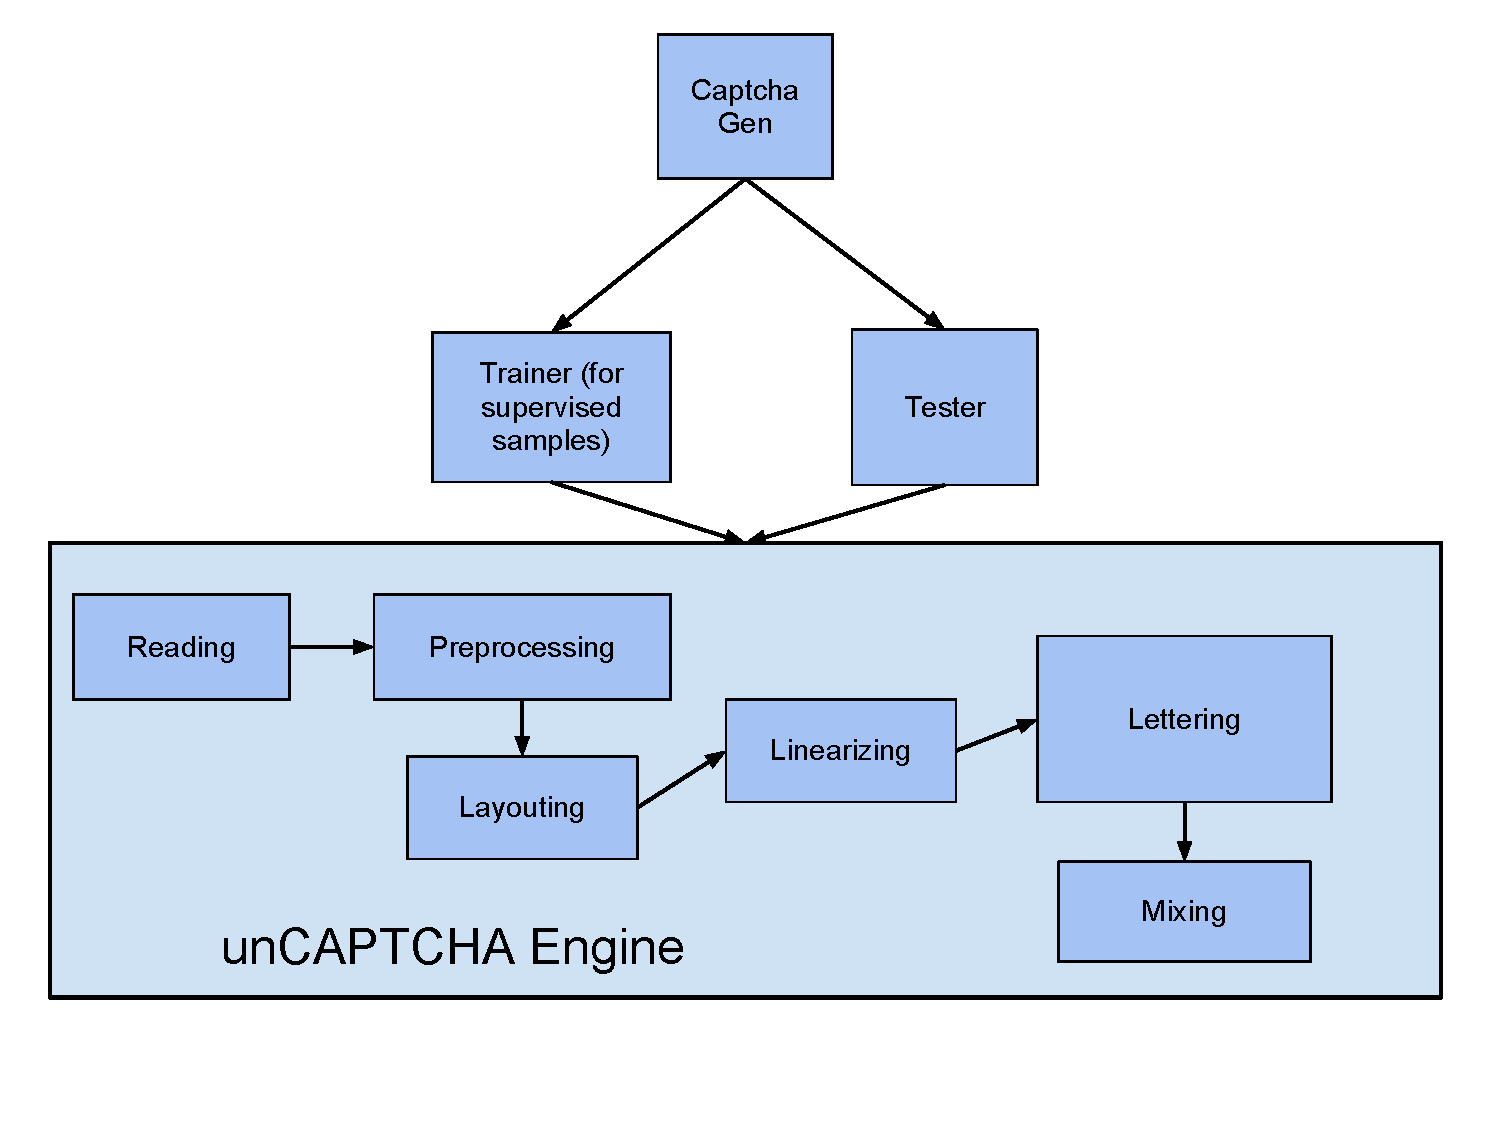
\includegraphics[width=0.85\textwidth]{img/unCAPTCHAarchitecturedraft.pdf}
\caption{unCAPTCHA architecture}
\label{fig:architecture}
\end{figure}
The application code will be constructed using a pipelined approach: the image
containing the captcha will be fed as input to the executable and the output
will be the text contained in the captcha, possibly annotated with some more
informations (certainty in the result for example). % TODO: decide

We don't want to limit the application to a single kind of captcha. Because of
this, the pipeline must be easily expandable with new stages or some stages
from this pipeline should be easily switched with others.

% TODO: decide how do implement modifiable pipeline

There are a few modules in the pipeline which should be kept, no matter what
kind of image is given as input. By module we convey a sequence of stages,
each of them being concerned with one part of the entire transformation chain
from the input image to the output text.

The first one of the modules -- \textit{Reading} -- will involve reading the
image and converting it to an internal format. The initial captcha can be a
PNG, a JPEG or a PPM image, it does not matter for the application. This
initial module will read the image and will convert it's content to the same
internal format, regardless of the initial format.

The second one of these modules is called \textit{Preprocessing} and will
transform the image using a set of filters and image transformation tools such
that the number of distortions will be reduced. We expect that the output of
this stage will be a more clearer image. However, since this stage has little
information to work on -- at this point we only know that the image consists
of text and some details about the transformations done to it -- we cannot
guarantee that this module will achieve a perfect looking image at the end: we
will need more processing down the pipeline.

Next, -- at the \textit{Layouting} stage -- we will try to learn a few more
characteristics of the image: main line of the text, estimate distance between
letters, size of letters, etc. This model of the image will be passed down the
pipeline to more stages than just the next one.

Then, the \textit{Linearizing} stage will use the informations from the
\textit{Layouting} one in order to transform the image again such that each
letter of the text can be easily separated from its neighbours and the entire
text is laid out linearly, with as few distortions as possible.

After this, another learning stage will be placed. The \textit{Lettering}
stage will try to construct a possible representation of each letter in the
image. We can either output a single guess for each letter or several guesses
together with our confidence in their values. As inputs, this module will also
receive the output of the \textit{Layouting} phase. This will help to discern
between letters, making it easier to avoid problems caused by neighbouring
characters.

The last stage of the application will involve mixing these predictions in
order to create estimates for the text in the image. We can use several mixing
strategies here. Thus, the \textit{Mixing} module is able to output either a
single string or a list of strings together with our confidence in the fact
that each one of them was a member of the initial captcha.

\vskip 0.2in
\bibliographystyle{plain}
\bibliography{bibliography}

\end{document}
